%!TEX root = mb.tex
\eat{
\begin{figure}[t]
  \centering
  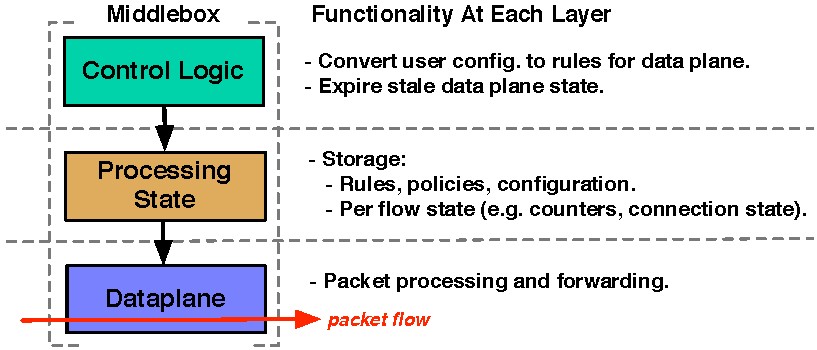
\includegraphics[width=3in]{fig/mbarch}
  \caption[]{\label{fig:mbarch} Typical middlebox software components. For most middleboxes, packet processing operations in the dataplane remain unmodified by \sys.}
\end{figure}
}
\section{Header-only middleboxes}
\label{sec:homiddleboxes}
% My high school english teacher would kill me for starting off a section without an introduction sentence. This is for him. HI MR KELLY.We now discuss how header-only middleboxes operate over the new encrypted packet format.
Most classes and functions within a middlebox codebase can be labeled as one of these three categories: the dataplane (which performs packet processing), the middlebox state (which stores and updates rules and policies, as well as per-flow state, and the control logic (which converts user configurations to rules and policies, and updates/refreshes state). 
Importantly, packet processing only occurs in dataplane functions, which are usually tightly engineered to process each packet in microseconds or faster.

As we will show, adapting middleboxes to operate over encrypted data requires (a) encrypting the rules given to the middleboxes, and (b) changes to the control logic and some of the processing state. 
However, the key algorithms that process packets on the dataplane remain unchanged for header-only middleboxes, with the exception of proxies.
This allows the packet-processing throughput to remain fast; as we see in our evaluation \S\ref{sec:eval} header-only middleboxes under \sys achieve near identical throughput to the same middleboxes over unencrypted data. 

\subsection{Middlebox: Firewall}\label{sec:firewall}

We use the term ``firewall'' for stateful and stateless packet filters that filter the traffic based on network layers and transport layers.
Our RangeMatch scheme supports both types of firewalls. We now explain the design of the firewall based on this scheme.

\noindent\textbf{Setup.} Initially, the gateway (G) encrypts the rules to be used by the firewall, by encrypting all IP addresses and ports in the rules, as follows.

First, it prepares the IP and port intervals. Recall that RangeMatch requires the IP addresses to be IPv6 to guarantee the injectivity of encryption (see \S\ref{sec:range}); hence, we extend an IPv4 prefix  such as 157.161.48.0/24 to an IPv6 one  ::ffff:157.161.48.0/120. 
% Now the prefix represents the range from ::ffff:157.161.48.0 to ::ffff:157.161.48.255.
This problem does not show up for ports because they only need to be distinct within the same IP address.
The gateway then expands every prefix into an interval, and every exact match $x$ into [$x$, $x$]. 

Next, the gateway encrypts these intervals using EncryptRanges (\S\ref{sec:range}) by running one instance of RangeMatch for IP addresses and one instance for ports.
It then converts each encrypted IP range into a set of prefixes and duplicates the rule for each prefix in this set. 

Consider an example rule from  \mf{pf}, the 
default firewall under BSD:
 \mf{ block out log quick on \$ext\_if from} \\ \mf{157.161.48.0/24 to any.}
 
Let the encryption of 157.161.48.0/24 be the interval [80.0.0.0, 160.0.0.0] (for brevity, we use IPv4). 
This interval is equivalent to the prefixes: 80.0.0.0/4, 96.0.0.0/3, 144.0.0.0/4, and 160.0.0.0/32. 
Hence, the gateway replaces the original rule with four rules, one for each encrypted prefix. 
The worst-case number of prefixes for IPv6 is $O$($\min$($\log$ number of rules, $128$)) = $O$($\log$ number of rules), 
which is small. 


% Firewalls from different vendors may vary significantly in terms of rule syntaxes and organizations. However,
% in general both hardware and software firewalls have a few interfaces. Both ingress and egress of an interface 
% can be associated with an access control list (ACL). Each ACL has a number of rules, possibly in the form 
% <action, protocol, src ip, src port, dst ip, dst port>. Without loss of generality, we take \mf{pf}, the 
% default firewall under BSD, as an example to illustrate how \sys works with firewalls. Figure \ref{fig:fwrule1} 
% shows an example of \mf{pf} rules. 





The gateway sends the new rules to the service provider (SP) which installs them into the firewall {\em the same way it would install 
them if they were not encrypted}. 

\noindent\textbf{Processing traffic.}
The gateway sends the packet to the firewall using the format described in \S\ref{sec:overview}. The firewall can execute on the encrypted header {\em
the same way as on the unencrypted header} because RangeMatch maintains the order relation between values in rules and in 
packet headers. 
In particular, it can use any of the existing fast matching algorithms unchanged. 
Further, many high-speed firewalls have a hardware datapath and these can be used without change.


\noindent\textbf{Updating rules.} 
When an administrator adds a new rule, the gateway computes the new values [$\enc(s), \enc(e)$] as well as a list of prefix changes based on $L$: this list maps old prefix to new prefix so that the firewall knows how to update its rules. 
The gateway sends the new rules and prefix changes to the firewall, and the firewall reconfigures itself. 
  Due to the guarantees of our RangeMatch protocol, this list contains a 
small number (logarithmic) of intervals that changed.
However, some firewalls keep per-flow state; if a packet's encryption changes due to a new rule, this state will no longer be usable.
We discuss how updates impact stateful middleboxes in \S\ref{sec:impl}.
\eat{
\noindent\textbf{Updating rules affects other middleboxes too.}
Since some encrypted ranges shifted, a previously encrypted IP address might now match wrong ranges.
This affects all the middleboxes that retained an encrypted IP address that matches the shifted ranges. 
Hence, the gateway sends a message to all the middleboxes saying that there was a range change. 

Consider any middlebox MB (which could be the firewall too). Whenever MB saves an encrypted IP address $\enc(v)$ as part of its state, MB has to save $\aes_k(v)$ as well.  Recall that each packet with $\enc(v)$ has $\aes_k(v)$ in its options header.

Now consider that  MB is informed that a range change occurred.  If MB's state  contains an encrypted IP address $\enc(v)$, this encryption has to be updated.  As a result,  MB sends $\enc(v)$ along with $\aes_k(v)$ to the gateway. The gateway decrypts $\aes_k(v)$ to obtain $v$, re-encrypts $v$ with EncryptValue and sends it back to MB. 
The same protocol happens for updates to ranges of ports. 


As an optimization, MB does not need to send all the encryptions  it holds. It can determine which encryptions need to be updated based on the range change that occurred, but we do not present these details here. 
}
Such adjustment of encryptions is inconvenient but it is  necessary for an encryption scheme like RangeMatch; without it, an impossibility result applies, as discussed in \S\ref{sec:range}. Nevertheless, this operation happens rarely and is not expensive: it happens only when firewall rules change and the number of ranges changed is  amortized logarithmic in the total number of ranges. 
 %\S\ref{sec:impl} describes how these updates are performed efficiently with minimal disruption of the traffic. 
 



\subsection{Middlebox: NAT}\label{sec:nat}






Instead of mapping unencrypted addresses/ports to public IP addresses/ports, the NAT maps IP addresses/ports that are {\em encrypted} to public IP addresses/ports. 
Consider an example: an encrypted private IP address ab12:342:: and encrypted private port 231 are mapped to a public IP address 160.1.1.1 with port 445.

The fast path of the NAT in \sys{} is unchanged from the regular NAT. 
When a packet arrives at the NAT with an encrypted   IP address of ab12:342:: and an encrypted port of 231, the NAT maps these to 160.1.1.1 and 445, and does the reverse for reverse traffic. 
This process proceeds the same as on unencrypted data because encrypted values look the same as unencrypted values. 
We discuss in \S\ref{sec:impl} what the NAT does when there are changes in the ranges stored at the firewall. 

%A difference is that the NAT must listen for announcements of range changes as will be discussed in  \S\ref{sec:impl}.
%For example, consider that the gateway announces a change of ranges for IP addresses.
%The NAT realizes that ab12:342:: might have become stale and sends it to the gateway along with the AES encryption. The gateway decrypts AES, obtains the original IP address, re-encrypts it with EncryptValue, informs the NAT of the new encryption 2e41:863:: and the NAT replaces  ab12:342:: with 2e41:863::.
%
%Because the NAT is stateful, it too must handle updates, as we describe in \S\ref{sec:impl}.

\subsection{Middlebox: Proxy/cache}\label{s:proxy}

The proxy  caches HTTP static content (e.g., images) in order to improve client-side performance. 
When a client opens a new HTTP connection, a typical proxy will capture the client's SYN packet and open a new connection to the client, as if the proxy were the web server. The proxy then opens a second connection in the background to the original web server, as if it were the client. 
When a client sends a request for new content, if the content is in the proxy's cache, the proxy will serve it from there. Otherwise, the proxy will forward this request to the web server and cache the new content. 

\noindent\textbf{Encryption at the gateway.} 
The gateway parses the HTTP header in a packet's payload to identify the file path $F$ in a ``GET'' request. 
This is easy to do because the header appears at the start of the payload. For this task, the gateway does negligible work, resulting in less than 1\% throughput loss over the RangeMatch encryption. 
Next, the gateway encrypts $F$ using the KeywordMatch scheme. In this case, it can use the deterministic version (discussed in~\S\ref{s:kwmatch}) with no reduction in security because the proxy caches a set of {\em unique} file paths. Hence, using this scheme, the gateway encrypts $F$ into $\aes_k(F)$ and places it into a packet sent on the metadata channel. %\clan{in the implementation section 7.1 we said we place it in a new packet sent over the metadata channel.} 
%Even though it examines the packet's payload, the gateway does not need per-connection state and can parse the HTTP header quickly, as we show in \S\ref{sec:eval}. 

\noindent\textbf{Processing at the proxy.} 
The proxy has a map of encrypted file path to encrypted file content. When the proxy receives a packet, the proxy extracts $\aes_k(F)$ from the options header and looks it up in the cache {\em as if it were not encrypted}. The use of deterministic encryption enables the proxy to use a fast search data structure/index, such as a hash map, unchanged. We have two cases: there is a hit or a miss. For hit, the proxy assembles a packet header for reverse traffic and attaches to it the encrypted file content from the cache. Even without being able to encrypt IP addresses or ports, the proxy can create the header by reversing the encrypted information in the original header.
For a miss, the proxy forwards the request to the web server. When receiving the response, the proxy caches it to serve future requests.

We can extend our proxy support to HTTP pipelining. %some connections bundle together in the same stream a bunch of HTTP requests. 
In this case,  an HTTP header may no longer appear at the beginning of a packet and it can appear in the middle of the packet or across packet boundaries. We do not give the details of our solution here, but at a high level, one can use the IDS approach in \S\ref{sec:ids} to enable the web proxy to search for keywords on the payload  (effectively parsing the HTTP header over encrypted data) and identify the encrypted file path. In this case though, \sys can no longer support the web proxy in the header-only mode; it becomes a bytestream-aware application. 























%
%
%OLD LONGER VERSION
%
%
%
%Instead of mapping unencrypted addresses/ports to public IP addresses/ports, the NAT maps IP addresses/ports that are encrypted to public IP addresses/ports. 
%Consider a very simple NAT example:
%
%\smallskip
%\small
%\noindent
%\begin{tabular}{c|c|c|c|c}
%encrypted IP   & encrypted  &  public IP   & public  &  AES   \\
%address           & port            &   address   &  port    & encryptions \\
%\hline
%ab12:342::               & 231                  & 160.1.1.1  &  445 &  [..] \\ 
%\end{tabular}
%\normalsize
%\smallskip
%
%The last column stores the AES encryptions corresponding to the first two columns. 
%
%The fast path of the NAT in \sys{} is unchanged from the regular NAT. 
%When a packet arrives at the NAT with an encrypted   IP address of ab12:342:: and an encrypted port of 231, the NAT maps these to 160.1.1.1 and 445, and does the reverse for reverse traffic. 
%This process proceeds the same as on unencrypted data because encrypted values look the same as unencrypted values. 
%
%
%A difference is that the NAT must listen for announcements of range changes as discussed in \S\ref{sec:firewall}.
%For example, consider that the gateway announces a change of ranges for IP addresses.
%The NAT realizes that ab12:342:: might have become stale and sends it to the gateway along with the AES encryption. The gateway decrypts AES, obtains the original IP address, re-encrypts it with EncryptValue, informs the NAT of the new encryption 2e41:863:: and the NAT replaces  ab12:342:: with 2e41:863::.
%
%Because the NAT is stateful, it too must handle updates, as we describe in \S\ref{sec:impl}.
%
%\subsection{Middlebox: Proxy/cache}\label{s:proxy}
%
%The proxy  caches HTTP static content (e.g., images) in order to improve client-side performance. 
%When a client opens a new HTTP connection, a typical proxy will capture the client's SYN packet and open a new connection to the client, as if the proxy were the web server. The proxy then opens a second connection in the background to the original web server, as if it were the client. 
%When a client sends a request for new content, if the content is in the proxy's cache, the proxy will serve it from there. Otherwise, the proxy will forward this request to the web server and cache the new content. 
%
%\noindent\textbf{Encryption at the gateway.} 
%The gateway parses the HTTP header in a packet's payload to identify the file path $F$ in a ``GET'' request. 
%This is easy to do because the header appears at the start of the payload. For this task, the gateway does negligible work, resulting in less than 1\% throughput loss over the RangeMatch encryption. 
%Next, the gateway encrypts $F$ using the KeywordMatch scheme. In this case, it can use the deterministic version (discussed in~\S\ref{s:kwmatch}) with no reduction in security because the proxy caches a set of {\em unique} file paths. Hence, using this scheme, the gateway encrypts $F$ into $\aes_k(F)$ and places it into a packet sent on the metadata channel. %\clan{in the implementation section 7.1 we said we place it in a new packet sent over the metadata channel.} 
%%Even though it examines the packet's payload, the gateway does not need per-connection state and can parse the HTTP header quickly, as we show in \S\ref{sec:eval}. 
%
%\noindent\textbf{Processing at the proxy.} The proxy has a map of encrypted file path to encrypted file content. When the proxy receives a packet, the proxy extracts $\aes_k(F)$ from the options header and looks it up in the cache {\em as if it were not encrypted}. The use of deterministic encryption enables the proxy to use a fast search data structure/index, such as a hash map, unchanged. We have two cases: there is a hit or a miss. For hit, the proxy assembles a packet header for reverse traffic and attaches to it the encrypted file content from the cache. Even without being able to encrypt IP addresses or ports, the proxy can create the header by reversing the encrypted information in the original header.
%For miss, the proxy forwards the request to the web server. When receiving the response, the proxy caches it for file path $\aes_k(F)$ to serve future requests.
%
%We can extend our proxy support to HTTP pipelining. %some connections bundle together in the same stream a bunch of HTTP requests. 
%In this case,  an HTTP header may no longer appear at the beginning of a packet and it can appear in the middle of the packet or across packet boundaries. We do not give the details of our solution here, but at a high level, one can use the IDS approach in \S\ref{sec:ids} to enable the web proxy to search for keywords on the payload  (effectively parsing the HTTP header over encrypted data) and identify the encrypted file path. In this case though, \sys can no longer support the web proxy in the header-only mode; it becomes a bytestream-aware application. 
%

%SOME POTENTIALLY USEFUL INFO
%
%we are focusing on the transparent proxy
%- discuss the kind of proxies we are focusing on
%
%proxies have two benefits: latency savings which aplomb gives you 
%and bandwidth savings, which aplomb does nogive you
% 
%L7 Proxy / Cache
%
%With pipelined requests, we don't have the header is always the first part of the packet. Instead, we need to {\it reconstruct the payload} to tell where to parse. This is where we need to use the other gatway. Otherwise, the functionality is exactly the same above -- only now we operate on the reconstructed payload rather than the first few bytes of the first packet.
%









%When a client initiates a connection to a web server, the proxy {\it terminates} the connection instead of allowing packets to ``pass through''.
%
%
%However, rather than encrypting fixed values at fixed locations, the \sys gateway parses the HTTP header to determine what data to encrypt.
%Nevertheless, as we show in \S\ref{sec:eval}, this parsing has a negligible overhead on gateway throughput -- less than 1\% when added in addition to the existing encryption required for Firewalling and NAT.
%We implement two versions of gateway encryption: one which uses the stateless gateway and can encode HTTP requests which are not pipelined, and one which uses the stateful gateway, which supports pipelined HTTP requests as well (we discuss the difference as follows).




